% Online Supplement to the Journal of Sports Economics submission
% "The Limits of Foresight in Coaching Hires." Self-contained: same 12pt Times
% / booktabs / longtable setup as the main manuscript. Sections and tables are
% numbered with an "S" prefix (S1, S2; Table S1, Table S2) per the journal's
% supplementary-material convention. Cross-references to the main text are given
% in prose, since this document compiles independently of the manuscript.
\documentclass[12pt,USenglish]{article}

\usepackage[utf8]{inputenc}
\usepackage[T1]{fontenc}
\usepackage[margin=1in]{geometry}
\usepackage{mathptmx}            % Times for text and math
\usepackage{microtype}
\usepackage{setspace}
\usepackage{graphicx}
\usepackage{booktabs}
\usepackage{array}
\usepackage{longtable}
\usepackage{amsmath}
\usepackage{amssymb}
\usepackage[hidelinks]{hyperref}
\usepackage[natbibapa]{apacite}  % APA 7th author-date; matches the main manuscript

% Supplementary-material numbering: S1, S2, ...; Table S1, ...; Figure S1, ...
\renewcommand{\thesection}{S\arabic{section}}
\renewcommand{\thetable}{S\arabic{table}}
\renewcommand{\thefigure}{S\arabic{figure}}

\doublespacing

\begin{document}

\title{Online Supplement to\\
``The Limits of Foresight in Coaching Hires:\\
Pre-Hire Predictability of Involuntary Separation and the\\
Internal-Promotion Hazard in the NFL''}

% Author identity is carried on the separate title_page.tex (blinded review).
\author{}
\date{}
\maketitle

\noindent This supplement provides the full feature reference, the data-construction and coding
decisions, the model configuration, and supporting classifications for the analysis.
Section~\ref{sec:supp_features} defines every candidate pre-hire feature outside the pooled
unit block, which the main text summarizes by family in its Table~1;
Section~\ref{sec:supp_unitstats} itemizes the component statistics of the pooled unit block
introduced in Section~3.2.1 of the main text; Section~\ref{sec:supp_construction} documents
how the sample, the outcome, the internal-hire indicator, franchise lineage, and structurally
missing values are constructed; Section~\ref{sec:supp_config} reports the hyperparameter
search spaces for the tuned models and the stability-selection settings;
Section~\ref{sec:supp_nonfiring} lists every stint coded as a voluntary-while-viable
departure, the competing event, with its category and a one-line justification; and
Section~\ref{sec:supp_winrate} reports the win-rate-by-tenure outcome-validity check. All
feature values are measured at or before the hire date.

\section{Feature Descriptions}
\label{sec:supp_features}

Table~\ref{supp:featuredefs} defines the 55 candidate pre-hire features outside the pooled
unit block, grouped by family; with the 26 retained unit statistics
(Section~\ref{sec:supp_unitstats}) they form the 81-feature candidate set. All values are
measured at or before the hire date. Throughout, ``NFL'' experience includes the American
Football League of 1960--69, a major league whose ten franchises are NFL franchises today
(Section~\ref{sec:supp_construction}). Indicators marked $^{\dagger}$ flag values that are
structurally undefined rather than unobserved; their role is explained in
Section~\ref{sec:supp_missing}.

{\footnotesize\singlespacing
\begin{longtable}{@{}l p{8.8cm}@{}}
\caption{Definitions of the candidate pre-hire features by family. The pooled-unit block is itemized separately in Table~\ref{supp:unitstats}. $^{\dagger}$Structural indicator (Section~\ref{sec:supp_missing}).}
\label{supp:featuredefs}\\
\toprule
Feature & Definition \\
\midrule
\endfirsthead
\multicolumn{2}{c}{\tablename~\thetable\ (continued)}\\[2pt]
\toprule
Feature & Definition \\
\midrule
\endhead
\midrule
\multicolumn{2}{r}{\footnotesize\itshape continued on next page}\\
\endfoot
\bottomrule
\endlastfoot
\multicolumn{2}{@{}l}{\emph{Core experience (8)}}\\[2pt]
Age at hire & Coach's age in years at the start of the stint \\
Prior HC stints & Number of previous NFL head-coaching stints \\
College position-coach years & Seasons as a college position coach \\
College coordinator years & Seasons as a college coordinator \\
College head-coach years & Seasons as a college head coach \\
NFL position-coach years & Seasons as an NFL position coach \\
NFL coordinator years & Seasons as an NFL coordinator, special teams included \\
NFL head-coach years & Seasons with an NFL head-coaching title, a season taken over mid-season included; interim titles excluded \\
\addlinespace
\multicolumn{2}{@{}l}{\emph{Career structure (19)}}\\[2pt]
NFL employers & Distinct NFL franchises the coach worked for before the hire (relocation-aware) \\
College employers & Distinct college employers before the hire \\
NFL career share & Share of prior coaching seasons spent at the NFL level \\
Age at first job & Age at the coach's first coaching job of any kind \\
Age at first NFL job & Age at the coach's first NFL coaching job; equal to age at hire when this hire is his first NFL job \\
Gap before hire & Seasons between the coach's last coaching job and this hire \\
Internal hire & Indicator: held any coaching role with the hiring organization in the season before the hire, with franchise identity resolved relocation-aware (mid-season takeovers: Section~\ref{sec:supp_internal}) \\
Years at hiring org & Consecutive seasons with the hiring organization immediately before the hire \\
Hired from OC role & Indicator: the coach's most recent prior job was offensive coordinator \\
Hired from DC role & Indicator: most recent prior job was defensive coordinator \\
Hired from position-coach role & Indicator: most recent prior job was position coach \\
Hired from head-coach role & Indicator: most recent prior job was head coach (NFL or college) \\
Hired from offensive role & Indicator: most recent prior job was on the offensive side of the ball \\
Hired from NFL-level role & Indicator: most recent prior job was at the NFL level \\
Ever NFL OC & Indicator: ever an NFL offensive coordinator \\
Ever NFL DC & Indicator: ever an NFL defensive coordinator \\
Ever interim HC & Indicator: held an interim head-coaching title in a prior NFL season \\
No NFL unit record$^{\dagger}$ & Indicator: never led an NFL unit (no offensive or defensive coordinator season, and no head-coaching season outside an interim year), so the pooled unit statistics and recent-form measures do not exist \\
No drive-era record$^{\dagger}$ & Indicator: has a unit record but none from seasons with drive and situational statistics (recorded from about 1999) \\
\addlinespace
\multicolumn{2}{@{}l}{\emph{Recent form (6)}}\\[2pt]
Final unit percentile & League percentile of the coach's own unit (offense as OC, defense as DC, point differential as HC) in his last ranked season \\
Average unit percentile & Mean of those unit percentiles across prior ranked seasons \\
Unit trajectory & Slope of the unit percentile over the last three ranked seasons; zero when only one ranked season exists \\
Average team-success percentile & Mean league percentile of team winning percentage across prior ranked seasons \\
Ranked seasons & Number of prior ranked seasons (interim titles excluded) \\
No trend$^{\dagger}$ & Indicator: exactly one ranked season, so no trajectory exists \\
\addlinespace
\multicolumn{2}{@{}l}{\emph{Hiring-team results (3)}}\\[2pt]
Turnovers forced & Hiring team's turnovers forced, standardized within season, averaged over its prior two seasons \\
Turnovers committed & Hiring team's turnovers committed, standardized within season, averaged over its prior two seasons \\
Playoff appearances & Hiring team's playoff appearances in its prior two seasons (0--2) \\
\addlinespace
\multicolumn{2}{@{}l}{\emph{Inherited team quality (4)}}\\[2pt]
Offensive SRS & Hiring team's offensive Simple Rating System in the season before the hire (points per game vs.\ average, schedule-adjusted) \\
Defensive SRS & Hiring team's defensive Simple Rating System in the season before the hire \\
Strength of schedule & SRS strength-of-schedule component in the season before the hire \\
SRS trajectory & Slope of the hiring team's overall SRS over the three seasons before the hire \\
\addlinespace
\multicolumn{2}{@{}l}{\emph{Inherited roster (11)}}\\[2pt]
Starting-QB value & Average Approximate Value of the team's listed starting quarterback(s) in the season before the hire \\
Roster value & Average Approximate Value per rostered player in that season \\
Starter value & Average Approximate Value per starter in that season \\
Starter experience & Average seasons of NFL experience among starters \\
Roster experience & Average seasons of NFL experience across the roster \\
Recent first-round picks & First-round picks in the three drafts before the hire \\
Premium draft capital & First- and second-round picks in the same three drafts \\
Offensive retention & Percent of the offensive players on the roster two seasons before the hire still on the roster in the season before it, at any position \\
Defensive retention & The same, for defensive players \\
No roster data$^{\dagger}$ & Indicator: roster data are unavailable for the season before the hire (hires in 1970; rosters begin in 1970) \\
No retention data$^{\dagger}$ & Indicator: the two consecutive rosters that retention compares are unavailable (hires in 1970--71) \\
\addlinespace
\multicolumn{2}{@{}l}{\emph{Organizational instability (4)}}\\[2pt]
Predecessor tenure & Consecutive seasons of the coach being replaced, the team's season-opening head coach in the prior season \\
Predecessor fired & Indicator: the predecessor's stint ended in involuntary non-retention, coded under the same protocol as the outcome (Section~\ref{sec:supp_lineage}) \\
Head coaches in prior decade & Distinct head coaches the organization employed in the previous ten seasons \\
Expansion franchise$^{\dagger}$ & Indicator: first head coach of an expansion franchise, which inherits no predecessor, record, rating, or roster \\
\end{longtable}
}

\section{Pooled Unit Statistics}
\label{sec:supp_unitstats}

The pooled unit block summarizes a coach's prior on-field production in 33 statistics, each measured for the unit the coach's role controlled and pooled across his qualifying role-seasons as described in Section~3.2.1 of the main text. For an offensive coordinator a statistic reflects his own offense, for a defensive coordinator the suppression of the opposing offense, and for a non-interim head coach his whole team. An interim year adds no head-coaching statistics, while a coordinator title held outright that season still counts on its own side (Section~\ref{sec:supp_internal}). Every value is standardized against its season's league distribution and oriented so that larger is better, with turnovers, interceptions, penalties, and turnover percentage sign-flipped accordingly. In seasons shared by two leagues (the AFL and NFL of 1960--69, and the AAFC and NFL of 1946--49), each team is standardized against its own league, because the leagues played separate schedules in different scoring environments. Table~\ref{supp:unitstats} lists the 33 statistics in their source order; the seven marked $^{\ast}$ are collapsed as redundant with a retained statistic, leaving the 26 that enter the 81-feature candidate set. The thirteen drive and situational statistics (drives through red-zone rate) are recorded only from about 1999; their absence for earlier records is flagged rather than filled (Section~\ref{sec:supp_missing}). The block-level ablations reported in the main text's results are fit on the full 33-statistic block.

{\footnotesize\singlespacing
\begin{longtable}{@{}l l@{}}
\caption{The 33 pooled unit statistics, each standardized by season and oriented so that larger is better. A defensive coordinator's seasons contribute the same quantities measured against the opposing offense.}
\label{supp:unitstats}\\
\toprule
Statistic & Description \\
\midrule
\endfirsthead
\multicolumn{2}{c}{\tablename~\thetable\ (continued)}\\[2pt]
\toprule
Statistic & Description \\
\midrule
\endhead
\midrule
\multicolumn{2}{r}{\footnotesize\itshape continued on next page}\\
\endfoot
\bottomrule
\endlastfoot
Points scored$^{\ast}$ & Points scored by the unit \\
Total yards$^{\ast}$ & Total yards gained \\
Yards per play & Yards gained per offensive play \\
Turnovers & Turnovers committed (sign-flipped) \\
First downs & First downs gained \\
Completions & Pass completions \\
Pass attempts & Pass attempts \\
Passing yards & Yards gained passing \\
Passing touchdowns & Touchdown passes \\
Interceptions$^{\ast}$ & Interceptions thrown (sign-flipped) \\
Net yards per attempt$^{\ast}$ & Net yards per pass attempt, sacks included \\
Passing first downs & First downs gained passing \\
Rush attempts & Rushing attempts \\
Rushing yards & Yards gained rushing \\
Rushing touchdowns & Rushing touchdowns \\
Yards per carry & Yards per rushing attempt \\
Rushing first downs$^{\ast}$ & First downs gained rushing \\
Penalties & Penalties committed (sign-flipped) \\
Penalty yards$^{\ast}$ & Yards lost to penalties (sign-flipped) \\
First downs by penalty & First downs awarded by opponents' penalties \\
Drives & Number of offensive drives \\
Scoring percentage & Share of drives ending in a score \\
Turnover percentage & Share of drives ending in a turnover (sign-flipped) \\
Time per drive & Average time of possession per drive \\
Plays per drive & Average plays per drive \\
Yards per drive & Average yards per drive \\
Points per drive$^{\ast}$ & Average points per drive \\
Third-down attempts & Third-down attempts \\
Third-down rate & Third-down conversion rate \\
Fourth-down attempts & Fourth-down attempts \\
Fourth-down rate & Fourth-down conversion rate \\
Red-zone attempts & Trips inside the opponent's twenty-yard line \\
Red-zone rate & Share of red-zone trips ending in a touchdown \\
\end{longtable}
}

\section{Data Construction and Coding Decisions}
\label{sec:supp_construction}

\subsection{Sample and outcome}
\label{sec:supp_sample}

The sample is every non-interim head-coaching hire from the 1970 AFL--NFL merger through 2025:
365 stints. The American Football League of 1960--69 is treated as a major league: its seasons
count toward a coach's experience, unit record, and franchise history, and pre-merger seasons
are standardized within league (Section~\ref{sec:supp_unitstats}). A coach already in charge
when the window opens is a continuing stint rather than a hire, so AFL head coaches in place in
1970 (for example Hank Stram, who had led the franchise since its first season, as the 1960
Dallas Texans) are excluded exactly as NFL
incumbents such as Tom Landry are. Mid-season interim caretakers who never opened a season as
head coach are excluded; an interim coach retained for the following season enters as a hire
in that season, with his partial interim season counted as prior experience.

Outcomes run through the 2026 hiring cycle. The source data end with the 2025 season, so the
fate of every stint still running in 2025 was coded by hand from contemporaneous reporting
under the protocol of the main text: nine of these coaches were fired during or after the 2025
season, one left voluntarily (Mike Tomlin; Table~\ref{supp:nonfiring}), and 22 were still in
charge at the start of the 2026 season and are administratively censored.

A losing record in a coach's final season codes his exit as a firing however it was described.
Of the 260 exits after a losing final season, 40 were mid-season firings recorded as such in
the coaching record. We screened the other 220 against contemporaneous reporting for two
exceptions: a death or health exit, coded voluntary (category C), and a retirement announced
before the team's final game of that season, coded voluntary (category B). Three stints
qualify. Don McCafferty died of a heart attack at home in July 1974, before his second season
with the Lions, John McKay announced in November 1984 that he would
step down at the season's end, and Mike Holmgren announced before the 2008 season that it
would be his last. A retirement announced only after the final game, as was Bud Grant's in
1985, remains a firing, as does a resignation announced in the wake of a losing record, such
as Rich Kotite's in 1996. Coaches who left a losing season for a college job (for example Lou
Holtz, Ray Perkins, Nick Saban, and Bobby Petrino) are coded as fired. So are three who moved
directly to another NFL head-coaching job after a losing season: Chuck Knox (Buffalo 1982,
to Seattle), Forrest Gregg (Cincinnati 1983, released at his request to coach Green Bay), and
Herm Edwards (New York Jets 2005, traded to Kansas City for a fourth-round pick).

\subsection{Internal hire and mid-season takeovers}
\label{sec:supp_internal}

A hire is internal when the coach held any coaching role with the hiring organization in the
season before the hire, with franchise identity resolved across relocations and renames. The
rule looks only at the immediately preceding season: a coach who left an organization and
later returned as its head coach is internal only if he was back with it the season before.

Mid-season takeovers need care because the source data list only ``Head Coach'' for a partial
season and drop whatever job the coach held earlier that same season. Because such a stint is
dated from the next full season, the partial season itself makes the prior-season rule code
every mid-season takeover as internal. Each of the 18 such cases in the sample was therefore
checked against contemporaneous sources (Table~\ref{supp:midseason}). Fourteen coaches were
inside the organization when chosen and are coded internal: seven were on the coaching staff
the season before, and seven more held a staff or front-office position, or coached the club's
minor-league affiliate, before taking over, as documented in the clubs' own media guides and
contemporaneous press. Four were hired from outside as permanent head coaches and are coded
external.

An interim year never adds head-coaching statistics to a coach's unit record. A season is an
interim year when the coach held an interim title in it; when he took over as head coach
during it, since most of such a season was coached by his predecessor; or when PFR credits
him with a head-coaching season that his record does not show him holding (Anthony Lynn's
one game as Buffalo's caretaker in 2016, listed under his coordinator title). A coordinator title held outright
that season still counts on its own side of the ball, so a defensive coordinator named interim
head coach keeps that season's defense and gains no offense; an interim coordinator title never
counts. Every such season still counts as coaching experience, and the ``ever interim HC''
indicator records interim head-coaching titles.

{\footnotesize\singlespacing
\begin{longtable}{@{}l l c p{5.4cm} l@{}}
\caption{The 18 mid-season takeovers in the sample. ``Takeover'' is the season the coach took over during; the stint is dated from the following season. Sources: club media guides and contemporaneous press.}
\label{supp:midseason}\\
\toprule
Coach & Team & Takeover & Before taking over & Coded \\
\midrule
\endfirsthead
\multicolumn{5}{c}{\tablename~\thetable\ (continued)}\\[2pt]
\toprule
Coach & Team & Takeover & Before taking over & Coded \\
\midrule
\endhead
\midrule
\multicolumn{5}{r}{\footnotesize\itshape continued on next page}\\
\endfoot
\bottomrule
\endlastfoot
\multicolumn{5}{@{}l}{\emph{On the team's staff the season before the takeover}}\\[2pt]
Charlie Waller & SD & 1969 & Offensive backfield coach & internal \\
Jim Ringo & BUF & 1976 & Offensive line coach & internal \\
Al Saunders & SD & 1986 & Receivers coach & internal \\
Art Shell & LA Raiders & 1989 & Offensive line coach & internal \\
Richard Williamson & TB & 1990 & Receivers coach, assistant head coach & internal \\
Jason Garrett & DAL & 2010 & Assistant head coach, offensive coordinator & internal \\
Leslie Frazier & MIN & 2010 & Assistant head coach, defensive coordinator & internal \\
\addlinespace
\multicolumn{5}{@{}l}{\emph{Inside the organization before the takeover (from media guides and press)}}\\[2pt]
J.D. Roberts & NO & 1970 & Head coach of the Saints' minor-league affiliate (Richmond); Saints scout and linebackers coach 1967--68 & internal \\
Ed Khayat & PHI & 1971 & Defensive line coach & internal \\
Harland Svare & SD & 1971 & General manager & internal \\
Sid Gillman & HOU & 1973 & Executive vice president and general manager & internal \\
John McVay & NYG & 1976 & Assistant coach (research and development) & internal \\
Tommy Hudspeth & DET & 1976 & Scout from 1974, then coordinator of personnel and scouting & internal \\
Homer Rice & CIN & 1978 & Quarterbacks coach & internal \\
\addlinespace
\multicolumn{5}{@{}l}{\emph{Hired from outside as permanent head coach}}\\[2pt]
Don Coryell & SD & 1978 & Fired by the Cardinals; no Chargers role & external \\
Raymond Berry & NE & 1984 & Out of football since 1981 & external \\
Marv Levy & BUF & 1986 & Out of coaching; no Bills coaching role & external \\
Ron Meyer & IND & 1986 & Fired by the Patriots in 1984 & external \\
\end{longtable}
}

\subsection{Predecessor and franchise lineage}
\label{sec:supp_lineage}

The predecessor is the coach being replaced: the franchise's season-opening head coach in the
season before the hire, so that neither an interim caretaker nor the new coach's own partial
season stands in for him. Franchise identity follows relocations and renames. The 1996
Baltimore Ravens took over the 1995 Cleveland Browns' roster, staff, and ownership, so the
Ravens' first hire inherits the 1995 Browns' record, rating, roster, and coaching history,
while the reactivated 1999 Browns inherit none of it. The expansion indicator is set from the
known list of expansion franchises' first head coaches (Seattle and Tampa Bay 1976, Carolina
and Jacksonville 1995, Cleveland 1999, Houston 2002).

Whether the predecessor was fired is coded under the same protocol as the outcome. For 333
of the 359 hires with a predecessor, his stint is itself in the sample and its outcome label
is reused. The remaining 26 predecessors held stints that began before 1970 (for example
Tom Landry and Chuck Noll), or are AFL incumbents outside the window; their exits were coded
by the same rules, 10 by a losing final season and 16 from earlier verdicts or contemporaneous
reporting. Overall roster retention, the pooled version of the offensive and defensive
retention rates, is not a separate candidate.

\subsection{Structurally missing values}
\label{sec:supp_missing}

No feature is imputed by a statistical model. Every missing value in the candidate set has a
structural cause, recorded by one of six indicators (marked $^{\dagger}$ in
Table~\ref{supp:featuredefs}): a coach who never led an NFL unit has no unit statistics or
recent form; a record from before about 1999 has no drive statistics; a coach with one ranked
season has no trajectory; an expansion franchise has no inherited situation; and rosters,
which begin in 1970, are unavailable for 1970 hires and do not support retention for 1970--71
hires. Two values are defined rather than missing: the unit trajectory is zero for a
single-season record, and the age at first NFL job is the age at hire when this hire is the
coach's first NFL job. The structurally missing values are set to a constant and modeled
alongside their indicator, as with pack-years of smoking for a never-smoker: the indicator
estimates the hazard of the group that lacks the measure, so the constant carries no
information and the coefficient on the measure is identified only from coaches who have it.
Whenever a feature enters a model, the indicators that mark its filled values enter with it.
After these indicators, no missing value in the candidate set remains unexplained.

No indicator is ever selected on its own. Three record when a data source begins rather
than anything a hiring team knew (no roster data, no retention data, and no drive-era
record), so selecting one would amount to selecting a hire-year indicator created by the
sources. The other three (no NFL unit record, expansion franchise, and a single ranked
season) mark rows where a feature does not exist; they are nuisance terms that let that
feature's coefficient come from the rows that have it, not findings. All six enter a model
only alongside the features whose values they mark. Stability selection therefore ranks 75
of the 81 candidate features.

\section{Model Configuration}
\label{sec:supp_config}

Table~\ref{supp:hyperparameters} reports the search spaces and selected values for the two tuned models. The Cox elastic-net penalty for the full candidate matrix, used to rank features and to fit the cross-validated comparison sets, was chosen by exhaustive grid search maximizing coach-level cross-validated concordance. The penalty for the stability-selected model was tuned the same way on its own columns, over the grid of the second panel, with ties going to the lightest penalty: a single binary feature ranks the stints identically at every penalty, so the lightest is used. The XGBoost-AFT benchmark was tuned by random search over 200 draws from the grid shown, making interaction structure up to depth five available to it. Both configurations were held fixed across the 50 resamples. The reported hazard-ratio model in the main text is unpenalized, for the inferential reasons given there, and the parametric AFT benchmarks use a small fixed ridge penalty ($0.01$).

Stability selection operates on the 75 selectable candidate features described in Section~\ref{sec:supp_features} (the six structural indicators of Section~\ref{sec:supp_missing} enter only alongside their features), drawing 2000 coach-level subsamples at 50\% sampling and retaining features with selection frequency at least 0.6 among the top 10 per subsample, with the selection profile also recorded at the top 15 and 20. All resampling uses an 80/20 coach-level train/test split. The expected number of falsely selected features is bounded by $\mathbb{E}[V] \leq q^2 / \{(2\pi - 1)\,p\}$ \citep{meinshausen2010}, with $p = 75$ the feature-pool size and $q$ the per-subsample shortlist length; the bound is finite only for $\pi > \tfrac{1}{2}$ and tightens as $q$ shrinks, which motivates the small shortlist and the $\pi = 0.6$ threshold. Recording the profile at $q \in \{10, 15, 20\}$, reported in the main text's stability-selection table, lets the conclusions be read against that otherwise conventional choice.

\begin{table}[!ht]
\caption{Hyperparameter search spaces and selected values for the two tuned models. The Cox elastic net was searched exhaustively; the XGBoost-AFT benchmark by 200-draw random search. Both were selected by coach-level cross-validated concordance and held fixed across the 50 resamples.}
\label{supp:hyperparameters}
\small
\begin{tabular}{@{}l l c@{}}
\toprule
Hyperparameter & Search space & Selected \\
\midrule
\multicolumn{3}{@{}l}{\emph{Cox proportional hazards (elastic net), full candidate matrix}}\\
Penalizer & \{0.001, 0.005, 0.01, 0.05, 0.1, 0.3, 0.5, 1.0, 2.0\} & 0.1 \\
$\ell_1$ ratio & \{0, 0.25, 0.5, 0.75, 1.0\} & 1.0 \\
\addlinespace
\multicolumn{3}{@{}l}{\emph{Cox proportional hazards (elastic net), stability-selected model}}\\
Penalizer & \{0.01, 0.05, 0.1, 0.5, 1.0\} & 0.01 \\
$\ell_1$ ratio & \{0, 0.5, 1.0\} & 0 \\
\addlinespace
\multicolumn{3}{@{}l}{\emph{XGBoost-AFT (normal AFT loss; 200 random draws)}}\\
Boosting rounds & \{30, 50, 80, 120, 200\} & 30 \\
Learning rate & \{0.02, 0.03, 0.05, 0.1, 0.15\} & 0.03 \\
Tree depth & \{2, 3, 4, 5\} & 4 \\
Row subsample & \{0.6, 0.7, 0.85, 1.0\} & 0.6 \\
Column subsample & \{0.6, 0.7, 0.85, 1.0\} & 0.85 \\
Minimum child weight & \{1, 3, 5, 8\} & 5 \\
$\ell_2$ regularization & \{0, 0.5, 1.0, 2.0, 5.0\} & 2.0 \\
AFT scale & \{0.5, 0.8, 1.0, 1.2, 1.5\} & 1.5 \\
\bottomrule
\end{tabular}
\end{table}

\section{Non-Firing Event Classifications}
\label{sec:supp_nonfiring}

Table~\ref{supp:nonfiring} lists every stint coded as a voluntary-while-viable departure, the competing event in our analysis, together with the category assigned under the competing-risks coding protocol of the main text and a one-line justification drawn from contemporaneous reporting. All terminated stints not listed here are coded as involuntary non-retention (firings); the conservative default-to-firing rule means a stint appears below only where positive evidence of a voluntary, while-viable exit was found. The 22 further non-firing stints not shown were still running at the start of the 2026 season and are administratively censored: Aaron Glenn, Andy Reid, Ben Johnson, Brian Schottenheimer, Dan Campbell, Dan Quinn, Dave Canales, DeMeco Ryans, Jim Harbaugh, Kellen Moore, Kevin O'Connell, Kyle Shanahan, Liam Coen, Matt LaFleur, Mike Macdonald, Mike Vrabel, Nick Sirianni, Sean McVay, Sean Payton, Shane Steichen, Todd Bowles, and Zac Taylor. Sean Payton appears here for his current stint and in Table~\ref{supp:nonfiring} for an earlier voluntary departure, the two being distinct stints. The outcomes of stints still running in 2025 were coded from 2026 reporting (Section~\ref{sec:supp_sample}).

{\footnotesize
\begin{longtable}{@{}l c c c p{7.6cm}@{}}
\caption{The 29 head-coaching stints coded as voluntary-while-viable departures (the competing event), grouped by category. Categories follow the main text's event-coding protocol: (A) departed for another head-coaching position while still wanted; (B) retired while still successful and retained, or announced his retirement before his final season ended; (C) departed for documented health, family, or other non-football reasons. ``Final (W--L)'' is the coach's record in his final season with the team.}
\label{supp:nonfiring}\\
\toprule
Coach & Stint & Final (W--L) & Cat. & Justification \\
\midrule
\endfirsthead
\multicolumn{5}{c}{\tablename~\thetable\ (continued)}\\[2pt]
\toprule
Coach & Stint & Final (W--L) & Cat. & Justification \\
\midrule
\endhead
\midrule
\multicolumn{5}{r}{\footnotesize\itshape continued on next page}\\
\endfoot
\bottomrule
\endlastfoot
\multicolumn{5}{@{}l}{\emph{(A) Departed for another head-coaching position while still wanted}}\\[2pt]
Chuck Fairbanks & 1973--1978 & 11--4 & A & Left for the University of Colorado head job \\
Jack Pardee & 1975--1977 & 9--5 & A & Resigned to take the Redskins head job \\
Bobby Ross & 1992--1996 & 8--8 & A & Left for the Lions head job; Chargers wanted to keep him \\
Bill Parcells & 1993--1996 & 11--5 & A & Left in a personnel dispute to take the Jets job \\
Mike Holmgren & 1992--1998 & 11--5 & A & Left for the Seahawks head coach and GM role \\
Al Groh & 2000 & 9--7 & A & Resigned to take the Virginia (alma mater) head job \\
Jon Gruden & 1998--2001 & 10--6 & A & Traded to Tampa Bay; remained a sought-after head coach \\
\midrule
\multicolumn{5}{@{}l}{\emph{(B) Retired while still successful and retained}}\\[2pt]
Sid Gillman & 1974 & 7--7 & B & Retired on top (Coach of the Year); picked his successor \\
John McKay & 1976--1984 & 6--10 & B & Announced in November 1984 he would step down at season's end \\
Bill Walsh & 1979--1988 & 10--6 & B & Retired days after winning Super Bowl XXIII \\
Jerry Burns & 1986--1991 & 8--8 & B & Announced his own retirement at 64; no pressure \\
Dick Vermeil & 1997--1999 & 13--3 & B & Retired after winning Super Bowl XXXIV \\
Bill Parcells & 1997--1999 & 8--8 & B & Retired on his own terms; Belichick set to succeed \\
Jimmy Johnson & 1996--1999 & 9--7 & B & Retired (burnout); Dolphins would have retained him \\
Dick Vermeil & 2001--2005 & 10--6 & B & Retired on top, still wanted \\
Bill Cowher & 1992--2006 & 8--8 & B & Stepped down after 15 seasons; SB winner the prior year \\
Bill Parcells & 2003--2006 & 9--7 & B & Retired by his own choice; the Cowboys wanted him back \\
Tony Dungy & 2002--2008 & 12--4 & B & Retired on top after a playoff run; picked his successor \\
Mike Holmgren & 1999--2008 & 4--12 & B & Announced before the 2008 season that it would be his last \\
Bruce Arians & 2019--2021 & 13--4 & B & Stepped down as a SB winner; picked successor Bowles \\
Sean Payton & 2006--2021 & 9--8 & B & Stepped away wanting time off; team would have kept him \\
\midrule
\multicolumn{5}{@{}l}{\emph{(C) Departed for health, family, or other non-football reasons}}\\[2pt]
Don McCafferty & 1973 & 6--7--1 & C & Died in office (heart attack at home, July 1974, before the season) \\
Bill Parcells & 1983--1990 & 13--3 & C & Resigned citing health after Super Bowl XXV \\
Joe Gibbs & 1981--1992 & 9--7 & C & Retired for health and family reasons \\
Bobby Ross & 1997--2000 & 5--4 & C & Resigned mid-season citing health (blood clots) \\
Joe Gibbs & 2004--2007 & 9--7 & C & Resigned for family reasons (grandson's illness) \\
Gary Kubiak & 2015--2016 & 9--7 & C & Retired for health reasons (migraine condition) \\
Bruce Arians & 2013--2017 & 8--8 & C & Retired citing family after a 42-year career \\
Mike Tomlin & 2007--2025 & 10--7 & C & Stepped down under contract and wanted back; owner described a family decision \\
\end{longtable}
}

\section{Outcome Validity: Win Rate by Tenure Length}
\label{sec:supp_winrate}

Longer tenures correspond to stronger regular-season records, which confirms that the modeled outcome, dismissal, tracks on-field success rather than chance variation in record.

\begin{figure}[!ht]
\centering
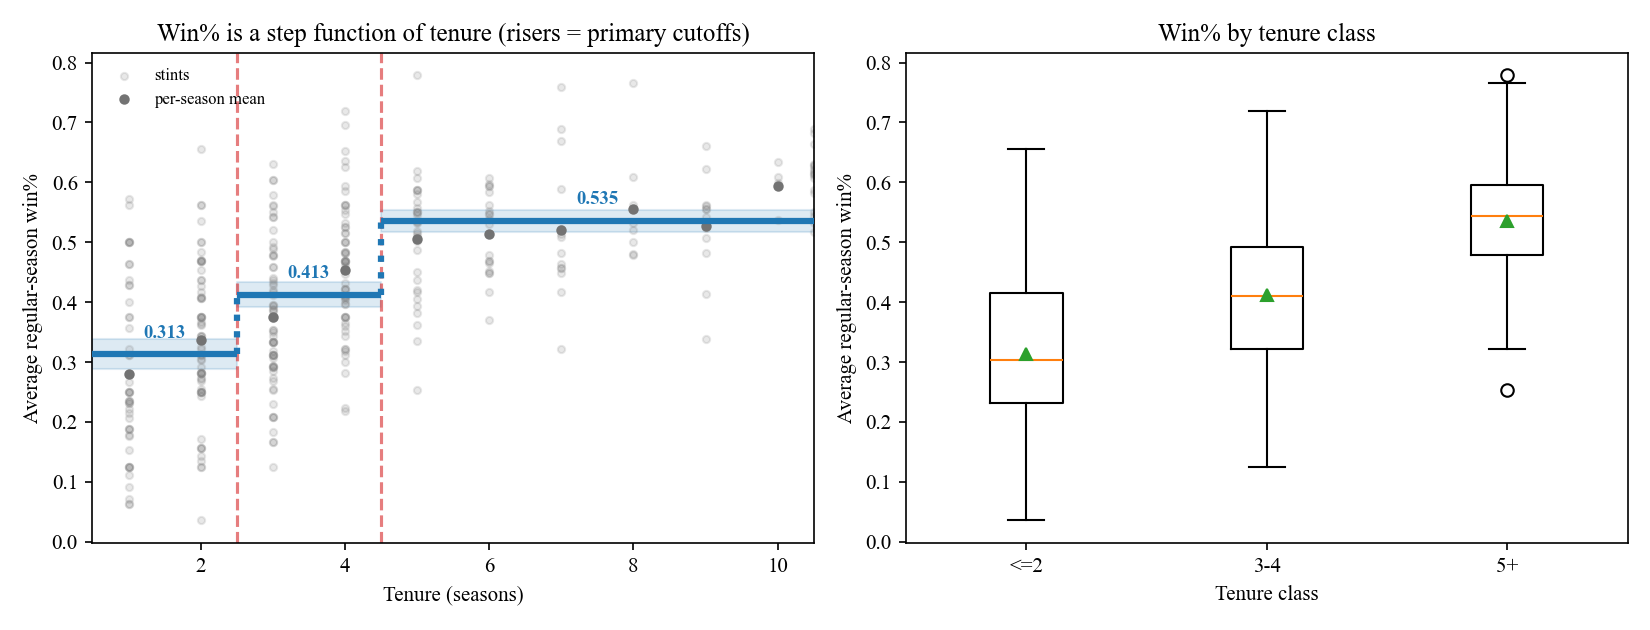
\includegraphics[width=0.75\textwidth]{figures/threshold_winrate.png}
\caption{Mean regular-season winning percentage by tenure length, which rises from 0.31 for short stints to 0.41 for medium and 0.54 for long (Kruskal--Wallis $p < 0.001$; each adjacent step ordered by a one-sided Mann--Whitney test, $p < 0.001$). Dismissal therefore tracks on-field success and is a meaningful outcome to model.}
\label{supp:winrate}
\end{figure}

\bibliographystyle{apacite}
\bibliography{refs}

\end{document}
